\documentclass[12pt, twoside]{article}
\usepackage{jmlda}
\usepackage{amsmath, amsfonts, amssymb}
\usepackage{pdfpages}
\newcommand{\hdir}{.}

\begin{document}

\title
    {Поиск границ радужки методом круговых проекций} % окончательное ли название?
\author
    {А.\,А.~Баженов, И.\,А.~Матвеев} % основной список авторов, выводимый в оглавление
\email
    {bazhenov.aa@phystech.edu; ivanmatveev@mail.ru}
%\thanks
%    {Работа выполнена при
%     %частичной
%     финансовой поддержке РФФИ, проекты \No\ \No 00-00-00000 и 00-00-00001.}
%\organization
%    {$^1$Организация, адрес; $^2$Организация, адрес}
\abstract
    {В работе рассматривается задача приблизительного нахождения границ радужки глаза. Входными данными являются изображение и считающееся известным положение зрачка глаза. Для нахождения границ зрачка и радужки используется нейронная сеть, для достижения максимальной производительности алгоритма используется предварительная обработка данных. Работа алгоритма проверена на базе изображений.
	
\bigskip
\noindent
\textbf{Ключевые слова}: \emph {}

}

%данные поля заполняются редакцией журнала
%\doi{10.21469/22233792}
%\receivedRus{01.01.2017}
%\receivedEng{January 01, 2017}

\maketitle
\linenumbers

\section{Введение}
Жизнь современного человека неразрывно связана с большим количеством аккаунтов, к каждому из которых необходим надежный способ аутентификации. Обзоры [1, 2] отмечают становление популярности биометрических способов идентификации человека относительно классических, таких как использование паролей. Обзор [2] особо выделяет методы, основанные на распознавании радужки, как позволяющие достигнуть высокой точности распознавания. Первичное выделение регионов на изображении глаза человека является одним из важнейших этапов персональной идентификации. В статье [3] описана общая схема работы системы сегментации изображения глаза: нахождение приблизительной позиции зрачка и последующее нахождение границ зрачка и радужки, с возможным итеративным уточнением.

В [3, 4] для реализации этапа первоначального определения границ радужки  используется метод круговых проекций. Круговая проекция яркости~--- интеграл градиента яркости изображения по окружности, имеющей центр в предполагаемом центре зрачка, либо по ее дуге. По предположению из [4], найдя точку локального максимума зависимости круговой проекции яркости от радиуса окружности, можно найти радиус границы радужки. Однако на яркость изображения в районе границы может оказываться влияние затемнения от ресниц и других элементов лица, что делает возможность эвристических алгоритмов, используемых в [3, 4] ограниченным.

Целью работы является исследование методов, которые возможно использовать для обработки результатов подсчета круговых проекций, причем более устойчивых к влиянию внешних факторов, чем эвристические алгоритмы. Один из таких методов~--- использование нейронной сети. Именно этом метод было решено исследовать в рамках работы.

\section{Постановка задачи}
\subsection{Модель системы нахождения границ радужки}

Рассматриваются данные в виде растрового изображения глаза $M$. Изображение представляет из себя зрачок~--- круг с центром в точке $\begin{pmatrix}P_x & P_y\end{pmatrix}^T$ и радиусом $P_R$, окруженный радужкой~--- кругом с центром в точке $\begin{pmatrix}I_x & I_y\end{pmatrix}^T$ и радиусом $I_R$, часть которого может отсутствовать на изображении.  Помимо зрачка и радужки, на изображении присутсвуют посторонние элементы.

Модель системы нахождения границ радужки представляется отображением $f\!: M \mapsto \begin{pmatrix}\widehat{P}_x & \widehat{P}_y & \widehat{P}_R & \widehat{I}_x & \widehat{I}_y & \widehat{I}_R\end{pmatrix}^T$. Для отбора моделей вводится функция потерь:
 \[
  L(x, y) = h\left(\frac{|x-y|}{x}\right).
 \]
 Функция $h(t)$ задается формулой:
\[
h(t) = (t-0.1) \cdot I_{[0.1; 0.2)}(t) + (5t-0.9) \cdot I_{[0.2; +\infty)}(t),
\] % возможно, не помешал бы график
где $I_A(x)$~--- индикаторная функция множества $A$. Рассматривается следующая задача оптимизации:
\begin{equation}
\sum_{i=1}^n   L\left(P_{Ri}, \widehat{P}_{Ri}\right)  + L\left(I_{Ri}, \widehat{I}_{Ri}\right) \to \min_f.
\end{equation}

\subsection{Метод круговых проекций}

Метод описан в статье [4]. Обозначим $\vec{x} = (x, y)$~--- точку на изображении, $b(\vec{x})$~--- яркость изображения в этой точке, $\vec{g}(\vec{x}) = \nabla b(\vec{x})$~--- градиент яркости. Согласно предположению, указанному в статье [4], точки, лежащие на границе радужки либо зрачка, должны удовлетворять условию, описываемому индикаторной функцией:
\[
v_U(\vec{x}) = \begin{cases}1, & \parallel \vec{g} \parallel > T_1 \land \frac{(\vec{x}, \vec{g})}{\parallel x \parallel \cdot \parallel g \parallel} > T_2 \land \vec{x} \in U, \\ 0, & \text{ иначе,}\end{cases}
\]
где $T_1$ и $T_2$~--- некоторые пороговые значения, а $U$~--- квадрант, то есть одно из множеств точек плоскости:
\[
U = \begin{cases}L\!: & |x| > |y| \land x < 0, \\ R\!: & |x| > |y| \land x > 0, \\ B\!: & |x| \leqslant |y| \land y < 0, \\ T\!: & |x| \leqslant |y| \land y > 0.\end{cases}
\]

Для аккумуляции значений индикаторных величин вводится следующее понятие. Пусть зафиксирован некоторый квадрант $U$. Тогда \textit{круговой проекцией яркости по окружности радиуса $r$} называется следующая величина:
\[
\Pi_U(r) = \frac{1}{2\pi r} \sum_{r-0.5 \leqslant \parallel x \parallel \leqslant r + 0.5} v_U(r).
\]
Радиус $r^*$, соответствующий границам зрачка и радужки, является точкой локального максимума функции $\Pi_U(r)$.

\subsection{Алгоритм поиска оптимального радиуса}

При известном приблизительном расположении зрачка встает задача поиска приблизительных радиусов границ радужки $\widehat{I}_R$ и зрачка $\widehat{P}_R$ при помощи некоторой модели. В работе в качестве таких моделей, выступают нейроные сети, принимающие как входные данные значения $\Pi_U(r)$, $U \in \{L, R, T, B\}$,  $r \in [0, r_{\max }] $, либо точки локальных максимумов функционала $\Pi_U(r)$, $U \in \{L, R, T, B\}$ и их значения. Обучение моделей есть решение задачи оптимизации:
\begin{equation}
\sum_{i=1}^n \left(\widehat{I}_{Ri} - I_{Ri}\right)^2 + \left(\widehat{P}_{Ri} - P_{Ri}\right)^2 \to \min_{f \in \mathbf{F}_k},
\end{equation}
где $\mathbf{F}_k$~--- некоторое подсемейство моделей. Обученные модели сравниваются с точки зрения качества решения задачи (1).

\section{Вычислительный эксперимент}

\subsection{Схема проведения эксперимента}

Проведение эксперимента заключается в оптимизации модели нейронной сети и последующем ее тестировании. Выборка изображений разделяется на три части: обучающую, валидационную и тестовую, размер которых относится как 4:1:1. Для всех изображений считаются круговые проекции яркости, считающиеся в дальнейшем исходными данными. При помощи алгоритмов оптимизации моделей строится модель $f$, являющаяся оценкой решения задачи (2).  Для промежуточных моделей, полученных на некоторой итерации решения задачи, подсчитывается функционал, используемый в задачах (1) и (2), на тестовой и валидационной выборках. Результат сравнивается со значениями для эвристического алгоритма. В конце эксперимента функционал (1) подсчитывается для тестовой выборки и сравнивается со значениями, получаемыми эвристическим алгоритмом.

\subsection{Цель эксперимента}

Целью работы является получение модели, результат которой превосходит результат работы эвристического алгоритма, при этом скорость получения предсказания должна позволять обрабатывать не менее 30 изображений в секунду.

\subsection{Результат эксперимента (предполагаемый)}

В процессе проведения эксперимента, описанного в предыдущем пункте получены значения функционала (2), отраженные на следующем графике:

\begin{center}
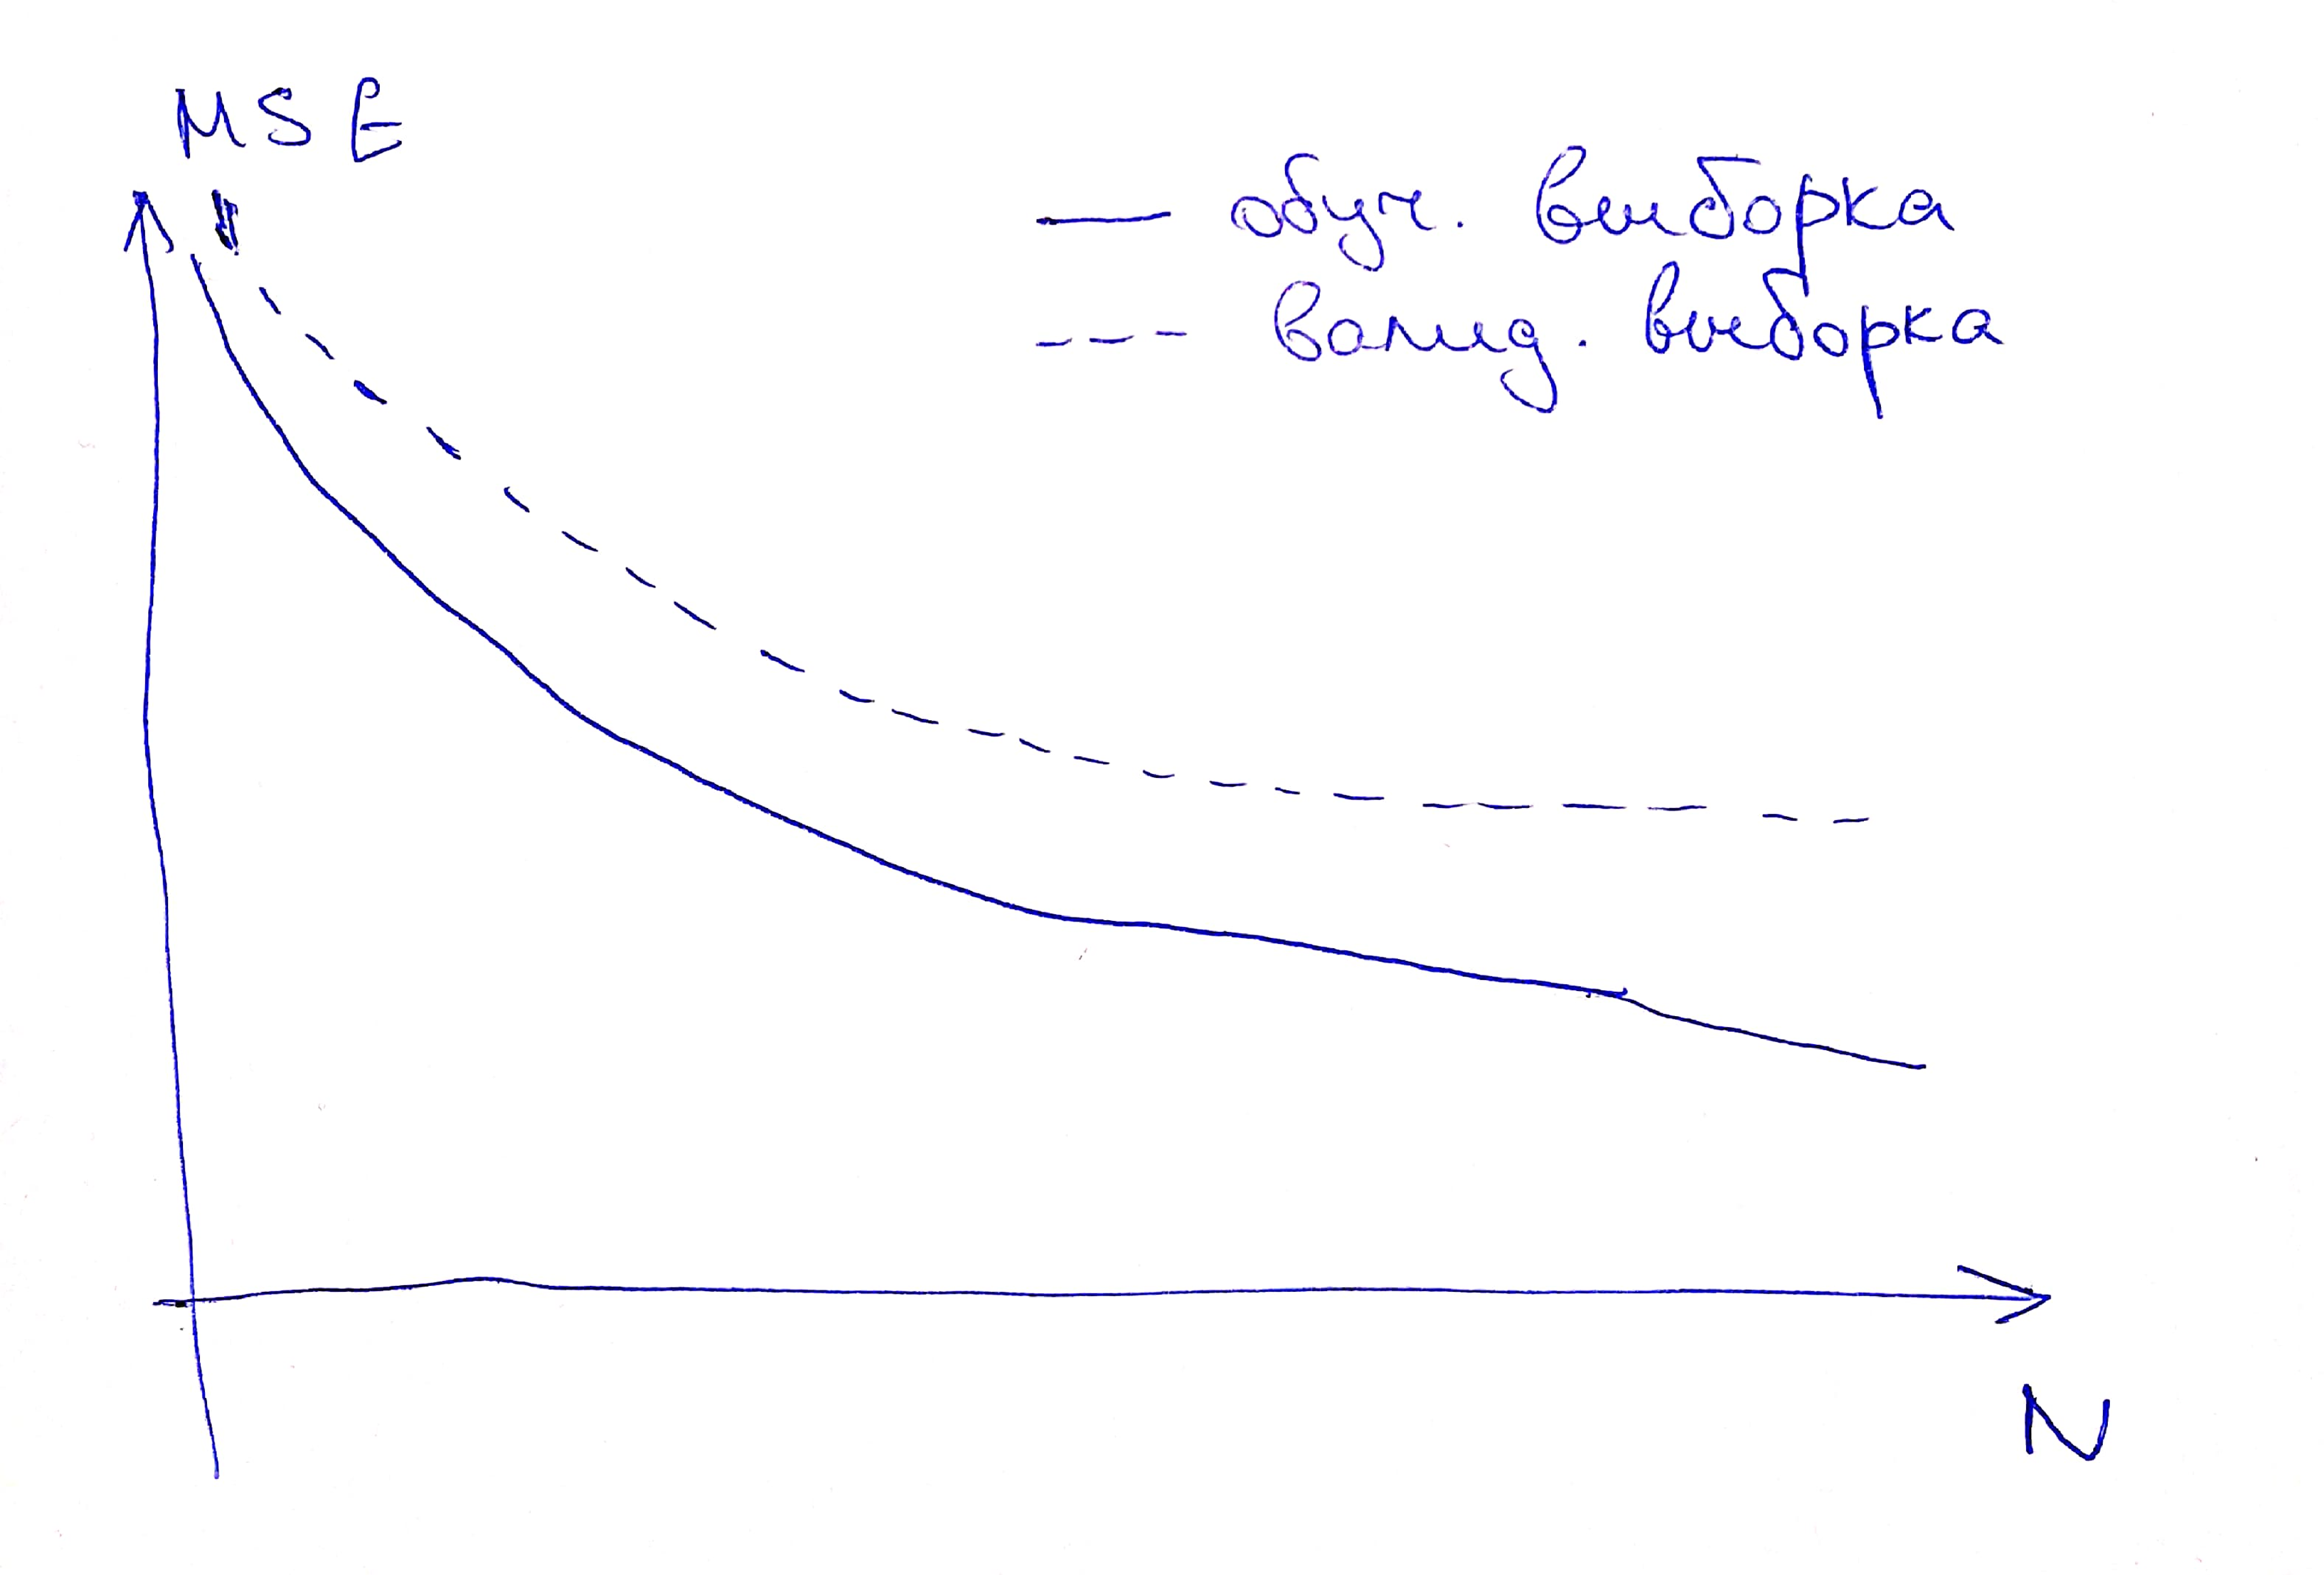
\includegraphics[width=7cm]{img/graph1.pdf}

Рис. 1. График зависимости функционала (2) от числа итераций обучения
\end{center}

Значения функционала (1) в сравнении с эвристическим алгоритмом приведены на следующем графике:
\begin{center}
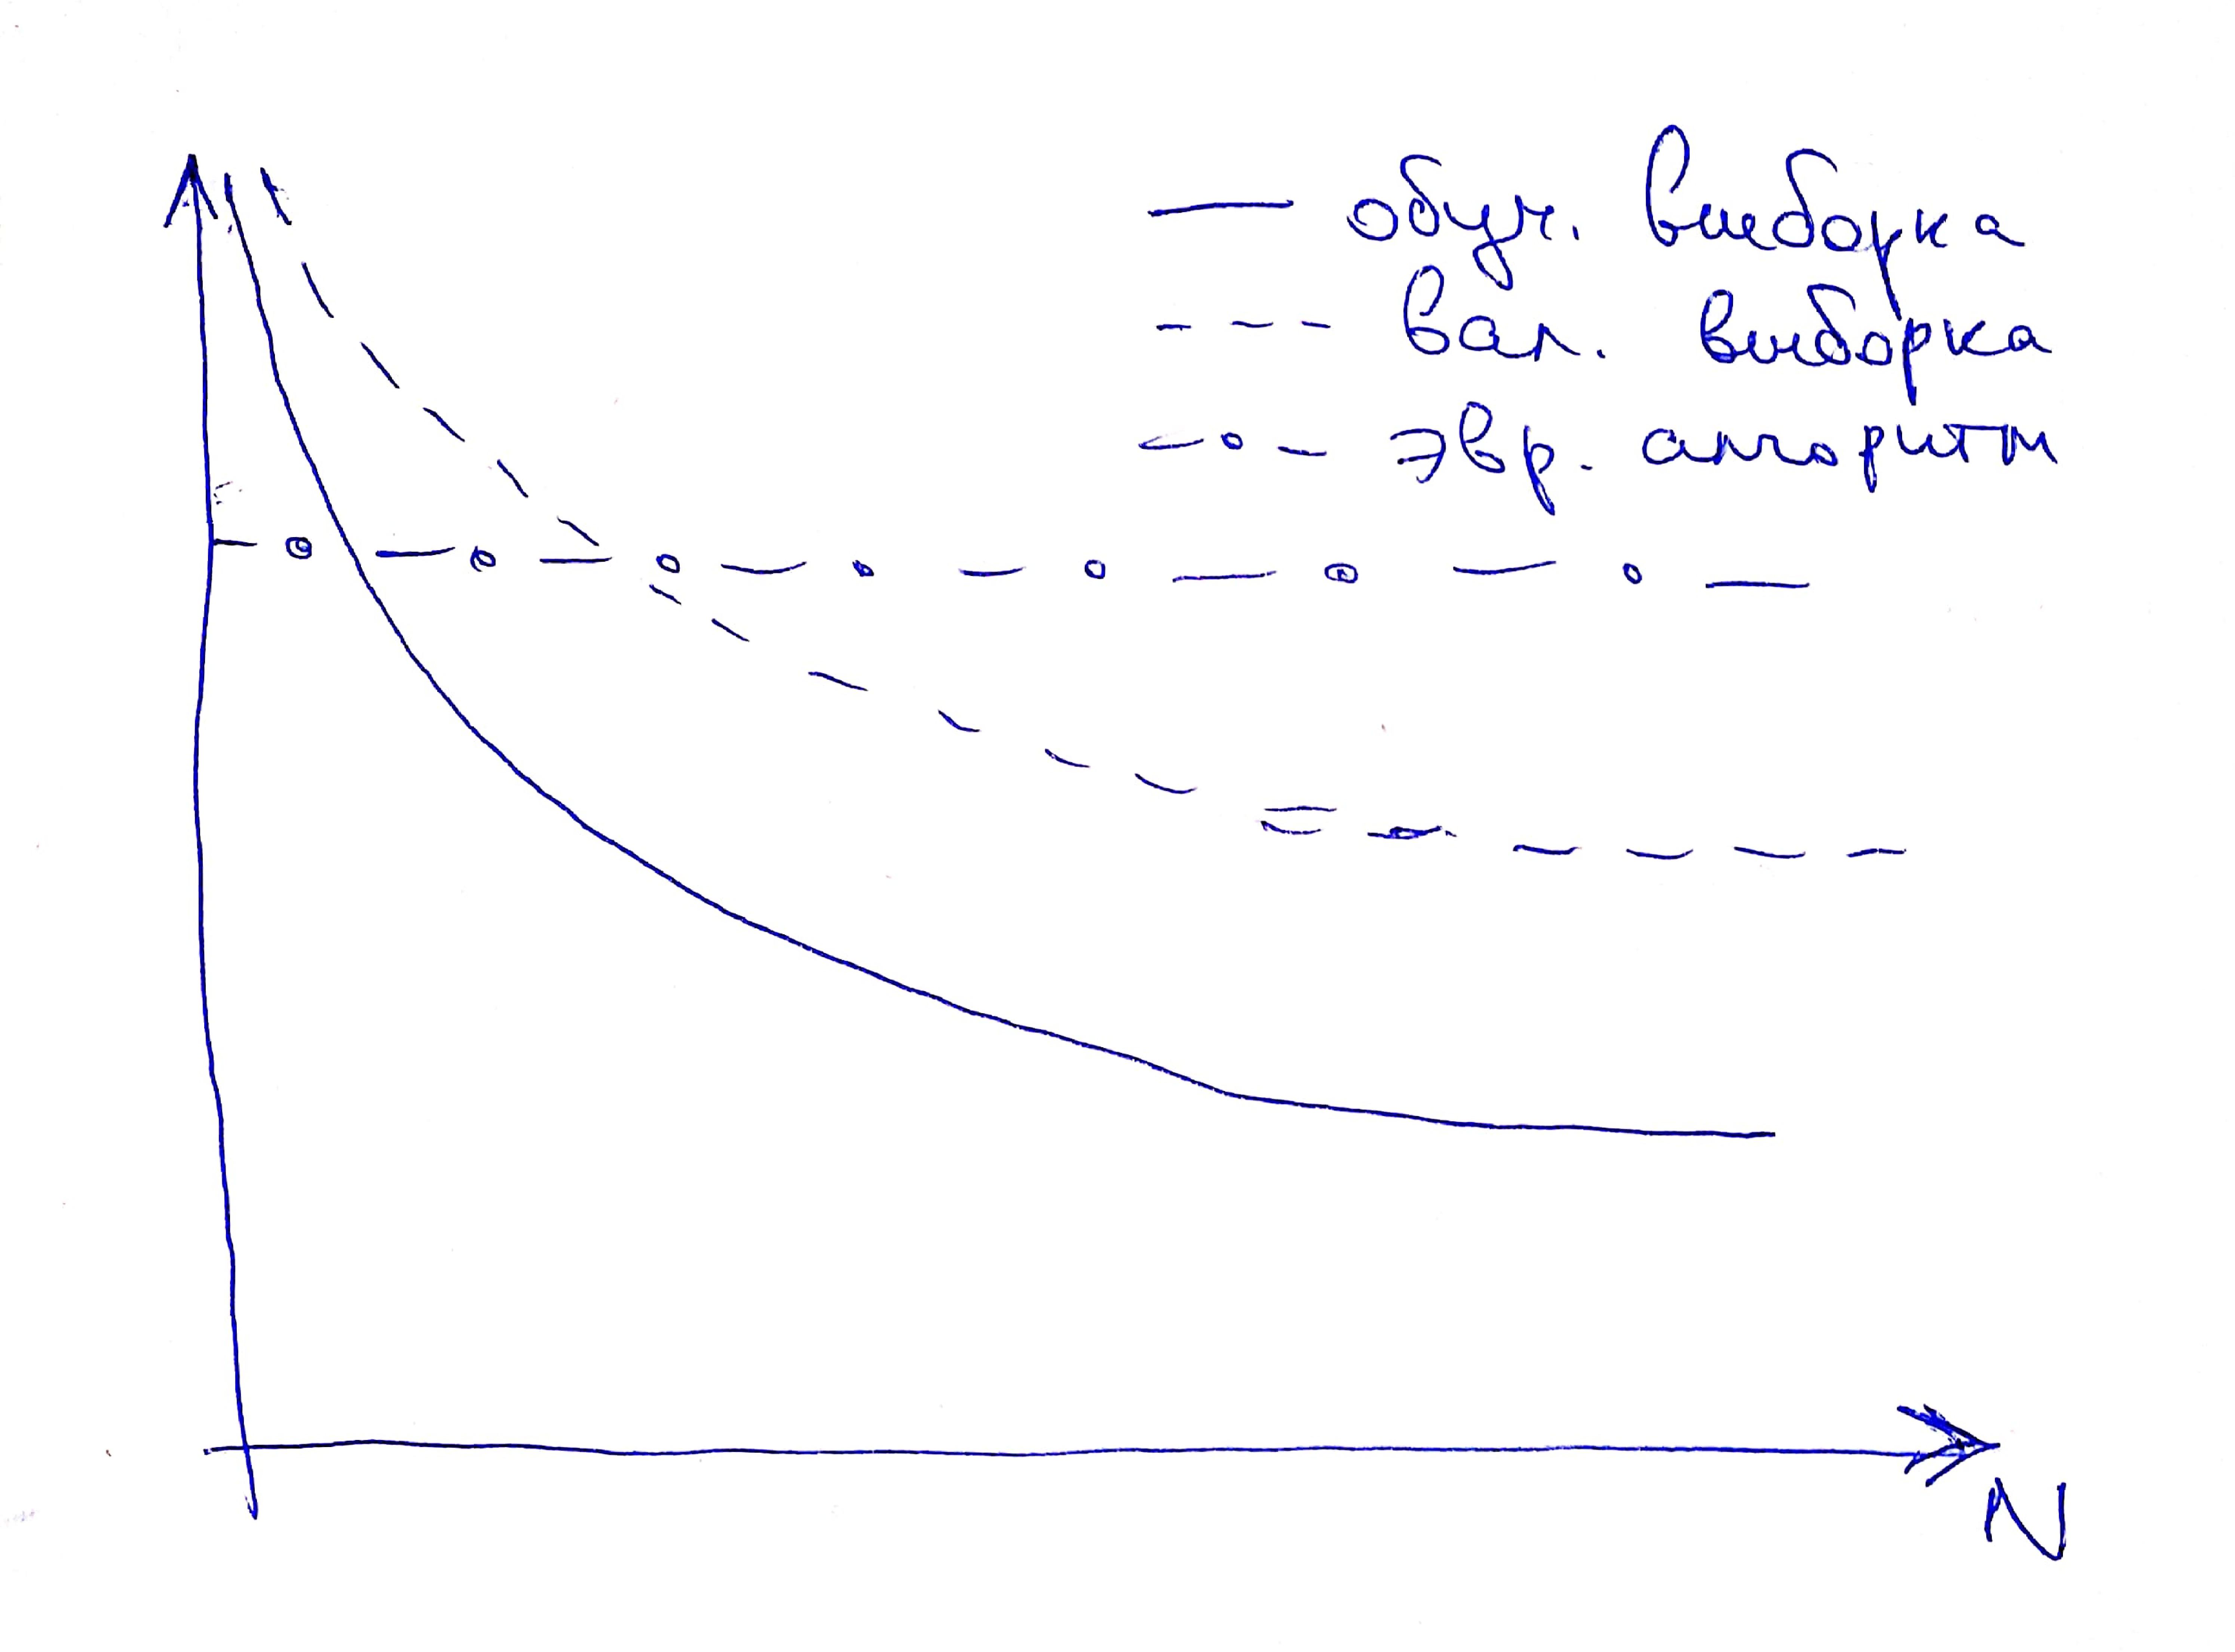
\includegraphics[width=7cm]{img/graph2.pdf}

Рис. 2. График зависимости функционала (1) от числа итераций обучения
\end{center}

Значение функционала (1) полностью обученной модели на тестовой выборке составило $F_1$, а эвристической модели~--- $F_2$.

%%%% если имеется doi цитируемого источника, необходимо его указать, см. пример в \bibitem{article}
%%%% DOI публикации, зарегистрированной в системе Crossref, можно получить по адресу http://www.crossref.org/guestquery/
\begin{thebibliography}{99}


 \bibitem{article}
    \BibAuthor{A.~Nithya, C.~Lakshmi}
   Iris Recognition Techniques: A Literature Survey~//
    \BibJournal{International Journal of Applied Engineering Research}, 2015

 \bibitem{article}
    \BibAuthor{K.~Bowyer, K.~Hollingsworth, and P.~Flynn}
   Image Understanding for Iris Biometrics: A Survey~//
    \BibJournal{Computer Vision and Image Understanding}, 2008. Vol.~110. \No\,2. pp.~281--307
	
 \bibitem{article} 
    \BibAuthor{K.\,A.~Gankin, A.\,N.~Gneushev, and I.\,A.~Matveev}
   Iris image segmentation based on approximate methods
with subsequent refinements~//
    \BibJournal{Journal of Computer and Systems Sciences International}, 2014. Vol.~53. \No\,2. pp.~224--238.
	\BibDoi{10.1134/S1064230714020099}.
	
  \bibitem{article}
    \BibAuthor{I.\,A.~Matveev}
   Detection of iris in image by interrelated maxima of brightness gradient projections~//
    \BibJournal{Appl. Comput. Math.}, 2010. Vol.~9. \No\,2. pp.~252--257.
	
 
 	
\end{thebibliography}

%%%% если имеется doi цитируемого источника, необходимо его указать, см. пример в \bibitem{article}
%%%% DOI публикации, зарегистрированной в системе Crossref, можно получить по адресу http://www.crossref.org/guestquery/.

\end{document}
